% TODO https://trello.com/
%
\chapter{Software Configuration Management}
Als Konfiguration eines Systems bezeichnet man die Festlegung seiner
Elemente mit ihren Versionen resp. Varianten:
(\href{http://www.software-kompetenz.de/?22704}
{www.software-kompetenz.de/?22704})
\begin{quote}
Eine Konfiguration ist ein Entwicklungsstand eines Produkts, in dem neben dem
Quellcode und der Dokumentation sämtliche Werkzeuge und Hilfsmittel zum
Erzeugen einer lauffähigen Version zusammengefasst sind. Das schließt auch die
Dokumentation und die Einstellungen bzw. verwendete Parameter der Werkzeuge
und Hilfsmittel ein.
\end{quote}
\newslide
Softwaresysteme sind aus vielfältigen Gründen \"Anderungen unterworfen:
Strategie- und Marketingentscheidungen, Fehlerbehebungen, Kundenforderungen,
nicht mehr unterstützte Softwareversionen von Drittherstellern etc.

\newslide
Änderungen betreffen meist unterschiedliche, von einander abhängige Elemente
\begin{itemize}
\item Anforderungskatalog, Spezifikation, Pflichtenheft
\item Designspezifikation
\item Testplan, Testreport, Testspezifikation
\item Projektplan
\item Quell-Kode
\item Makefiles
\item Produkte von Drittherstellern (Compiler, Libraries, Datenbank \ldots)
\item Benutzerhandbuch, Administrationsanweisungen
\item Ausbildungsunterlagen, Marketingbrochuren,
\item \ldots
\end{itemize}
Unkontrolliert durchgeführte Änderungen an einem oder mehreren Elementen
können unversehends zu Funktionsstörungen oder anderen Inkonsistenzen
führen.

Deshalb: Um die Integrität und Rückverfolgbarkeit eines Softwaresystems zu
gewährleisten, muss ein
systematischer Änderungsprozess betrieben werden:
\begin{quote}
Configuration Management ... is a management process for establishing and
maintaining consistency of a product's performance, its functional and
physical attributes, with its requirements, design and operational
information, throughout its life. (ANSI/EIA)
\end{quote}
\newpage
\section{Gliederung (IEEE/SWEBOK)}
\begin{figure}[H]
\centering
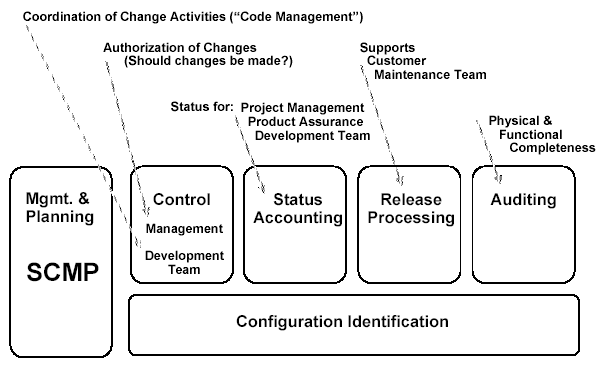
\includegraphics[width=0.75\linewidth]{config-management/scm-activities}
\caption{Software Configuration Management (Source: SWEBOK)}
\end{figure}
\begin{itemize}
\item \underline{SCMP}
   (Management des Software-Konfigurationsprozesses):
  \begin{itemize}
  \item Organisatorischer Kontext: Einbindung in die betriebliche
  Organisation, Bezeichnung der Schnittstellen und Verantwortlichkeiten,
\item Randbedingungen und Wegleitung: Berücksichtigung juristischer,
  ökonomischer, unternehmenspolitischer Faktoren, Anwendung von
  ``Best-Practices''
\item Planung: Festlegung und Anpassung der Verfahren und Werkzeuge zur
  Identifikation der Software-Elemente, Steuerung und Überwachung des
  Prozesses, Release-Management und Auslieferung, unter Berücksichtigung des
  Projektumfanges
  \end{itemize}
\item \underline{Configuration Identification} (Identifikation):
 Festlegung und Beschreibung der Bezugskonfiguration (Baseline),
  Markierung der Elemente, Aufnahme in die Konfiguration,
  Zulassungsverfahren (approval), Bezeichnung der Software-Bibliotheken
\item \underline{Control} (Steuerung):
  formelle Organisation und Behandlung von Änderungen,
  Strukturierung der Anfragen (Requests), Abschätzung der Auswirkungen,
  Durchführung und Freigabe, Umgang mit Abweichungen (Verzichtserklärungen)
\item \underline{Status Accounting} (Buchführung): Aufzeichnung der Aktivitäten mit
  Terminangaben und
  kommentierenden Erläuterungen, Ablageverfahren, Berichterstattung
\item \underline{Auditing} (Überwachung): Einhaltung der Vorgaben,
  Durchführung von Audits
%Evaluation von Verbesserungen
\item \underline{Release Processing} (Release-Managemement und Auslieferung):
  Festlegung,
  Erstellung und
  Beschreibung der auszuliefernden Konfiguration (Release Notes: neue
  Funktionalität, bekannte
  Einschränkungen und Probleme, Plattform-Anforderungen), Mitteilung an Kunden
\end{itemize}
%\newpage
%----------------------------------------------------------------------
\section{Versionen, Revisionen und Ausgaben}
Ein File (Dokument) kann verschiedene Versionen haben:
\begin{figure}[H]
\begin{center}
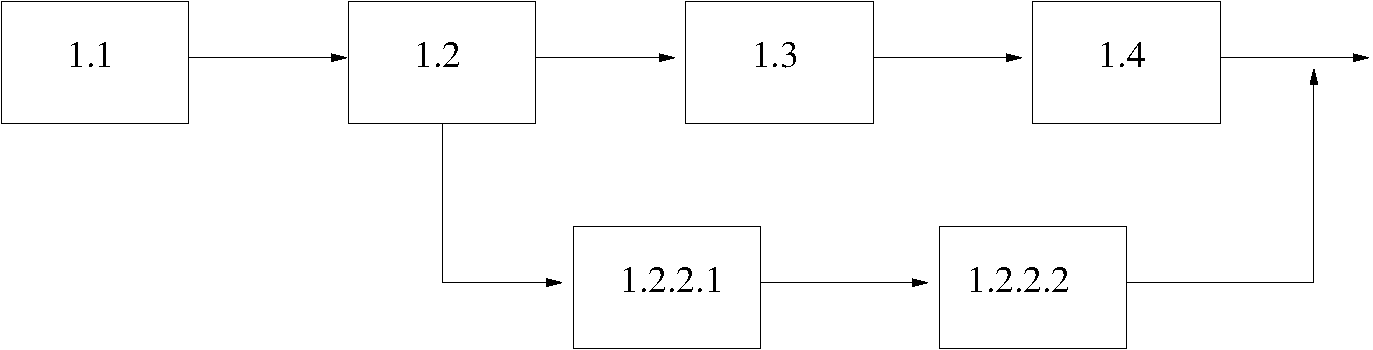
\includegraphics[width=0.8\linewidth]{config-management/xfig/file-revisions}
\end{center}
\caption{Die Versionen einer Datei}
\end{figure}
Sie werden \underline{Revisionen} (engl. Revisions) genannt.

\ifslides
\else
Ebenso kann ein Softwareprodukt mehrere Versionen haben. Man
nennt sie \underline{Ausgaben} (engl. Releases). Ihre Sourcefiles
haben jedoch unterschiedliche Versionen:

\fi
\begin{figure}[H]
\begin{center}
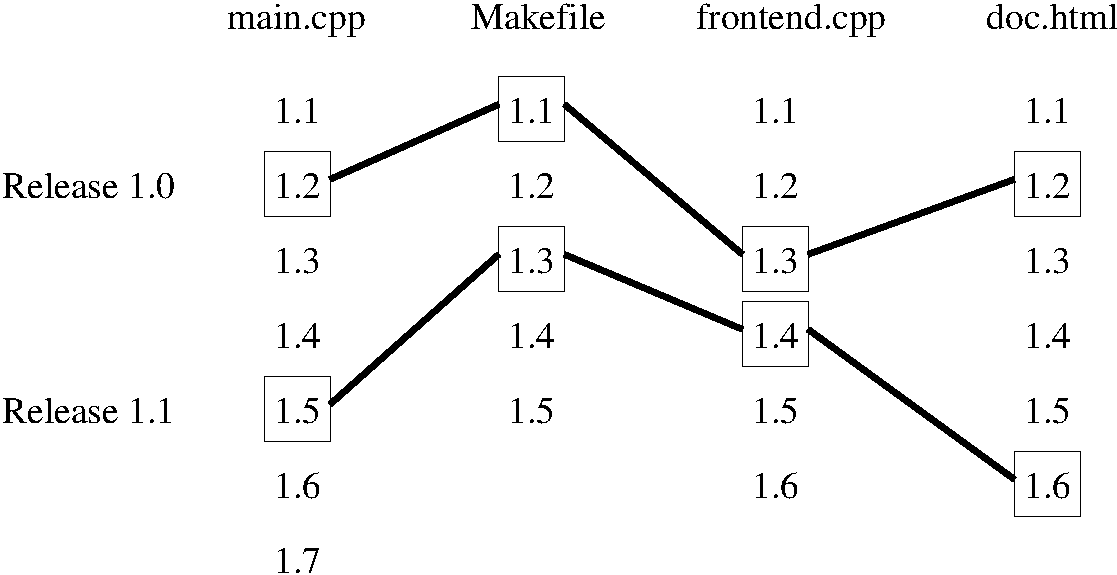
\includegraphics[width=0.9\linewidth]{config-management/xfig/releases}
\end{center}
\caption{Die Versionen eines Produktes}
\end{figure}
\newslide

Die Entwicklung erfolgt normalerweise entlang des Hauptastes
(Trunk oder Master). In mehreren Zyklen werden Dateien modifiziert,
hinzugefügt, gelöscht und umbenennt.

Bevor ein neuer Release gebildet wird, empfiehlt es sich
eine Verzweigung (Branch) zu erstellen. Dieser Moment wird auch als
``Code'' resp. ``Feature freeze'' bezeichnet, da innerhalb dieser Verzweigung
keine funktionalen Erweiterungen sondern nur noch diejenigen
Änderungen durchgeführt werden, die für die Integrations- und
Systemtests nötig sind. Nach Abschluss dieser Phase sollten die
Änderungen wieder mit dem Hauptast zusammengeführt werden.
\begin{figure}[H]
\begin{center}
  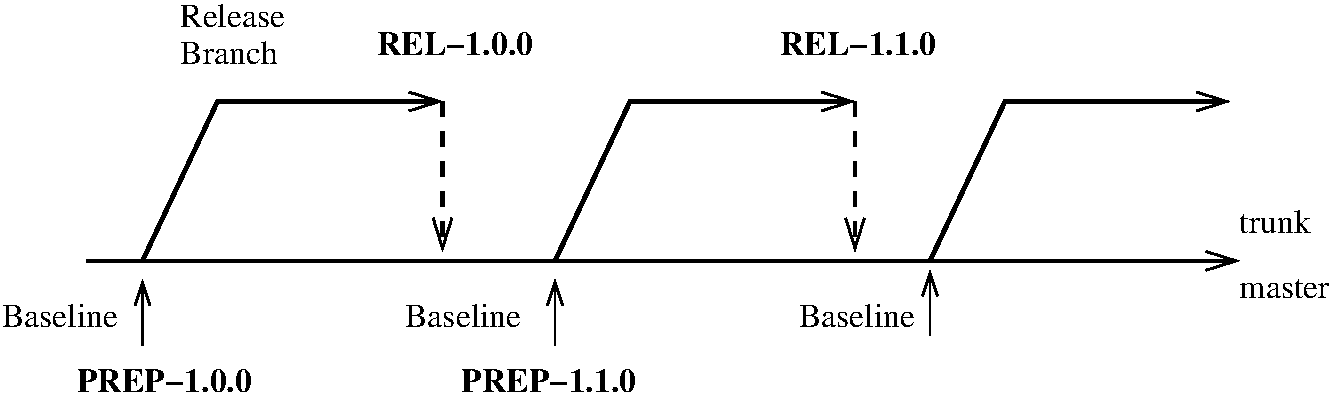
\includegraphics[width=0.9\linewidth]{config-management/xfig/release-branch}
\end{center}
\caption{Release-Bildung mit Branches und Merges}
\end{figure}
Die nicht mit dem Release beschäftigten Entwickler können während der
Release-Bildung auf dem Trunk weiterarbeiten.

\newslide
Für die Release-Bezeichnung empfiehlt es sich, ein einfaches und
nachvollziehbares Schema
anzuwenden. Z. B: {\bfseries major.minor.patch}

\begin{tabular}{ll}
Major: & umfangreiche Änderungen oder Erweiterungen\\
Minor: & zusätzliche Funktionalitäten\\
Patch: & Fehlerbehebungen oder geringfügige Verbesserungen\\
\end{tabular}

% Siehe http://apr.apache.org/versioning.html
%---------------------------------------------------------------
\newpage
%\subsection*{Konfigurationsmanagement}
\section{Change Management}
\begin{figure}[H]
\ifslides
\begin{center}
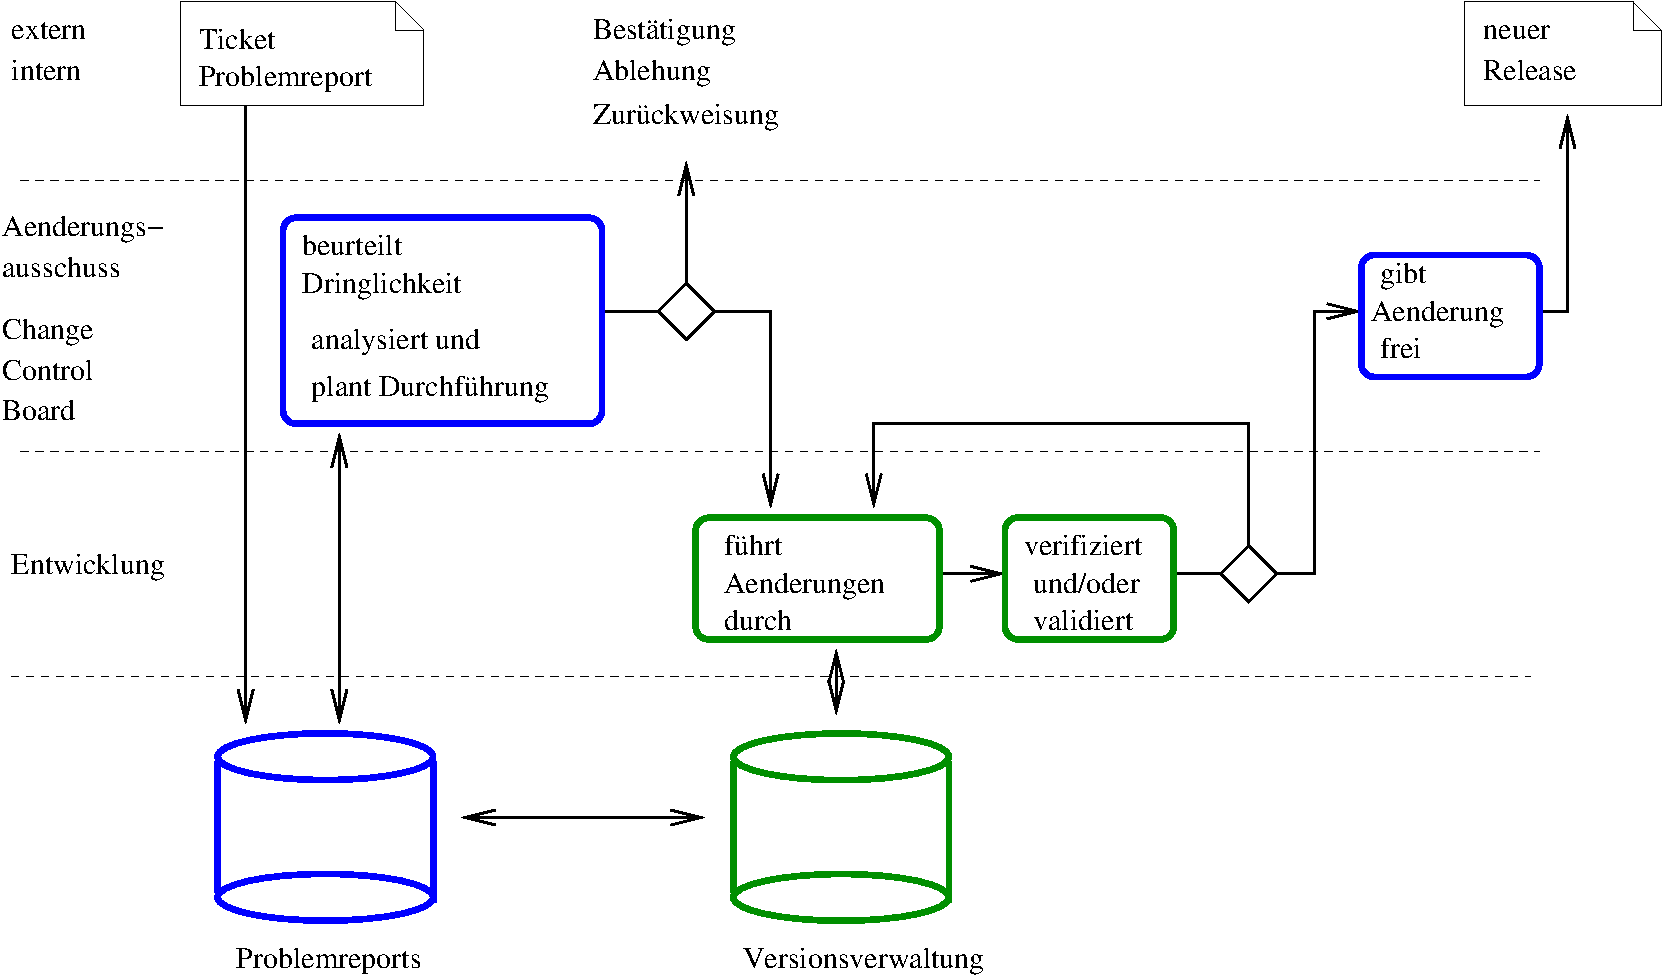
\includegraphics[width=0.65\linewidth]{config-management/xfig/changemgmt}\\[2ex]
\end{center}\else
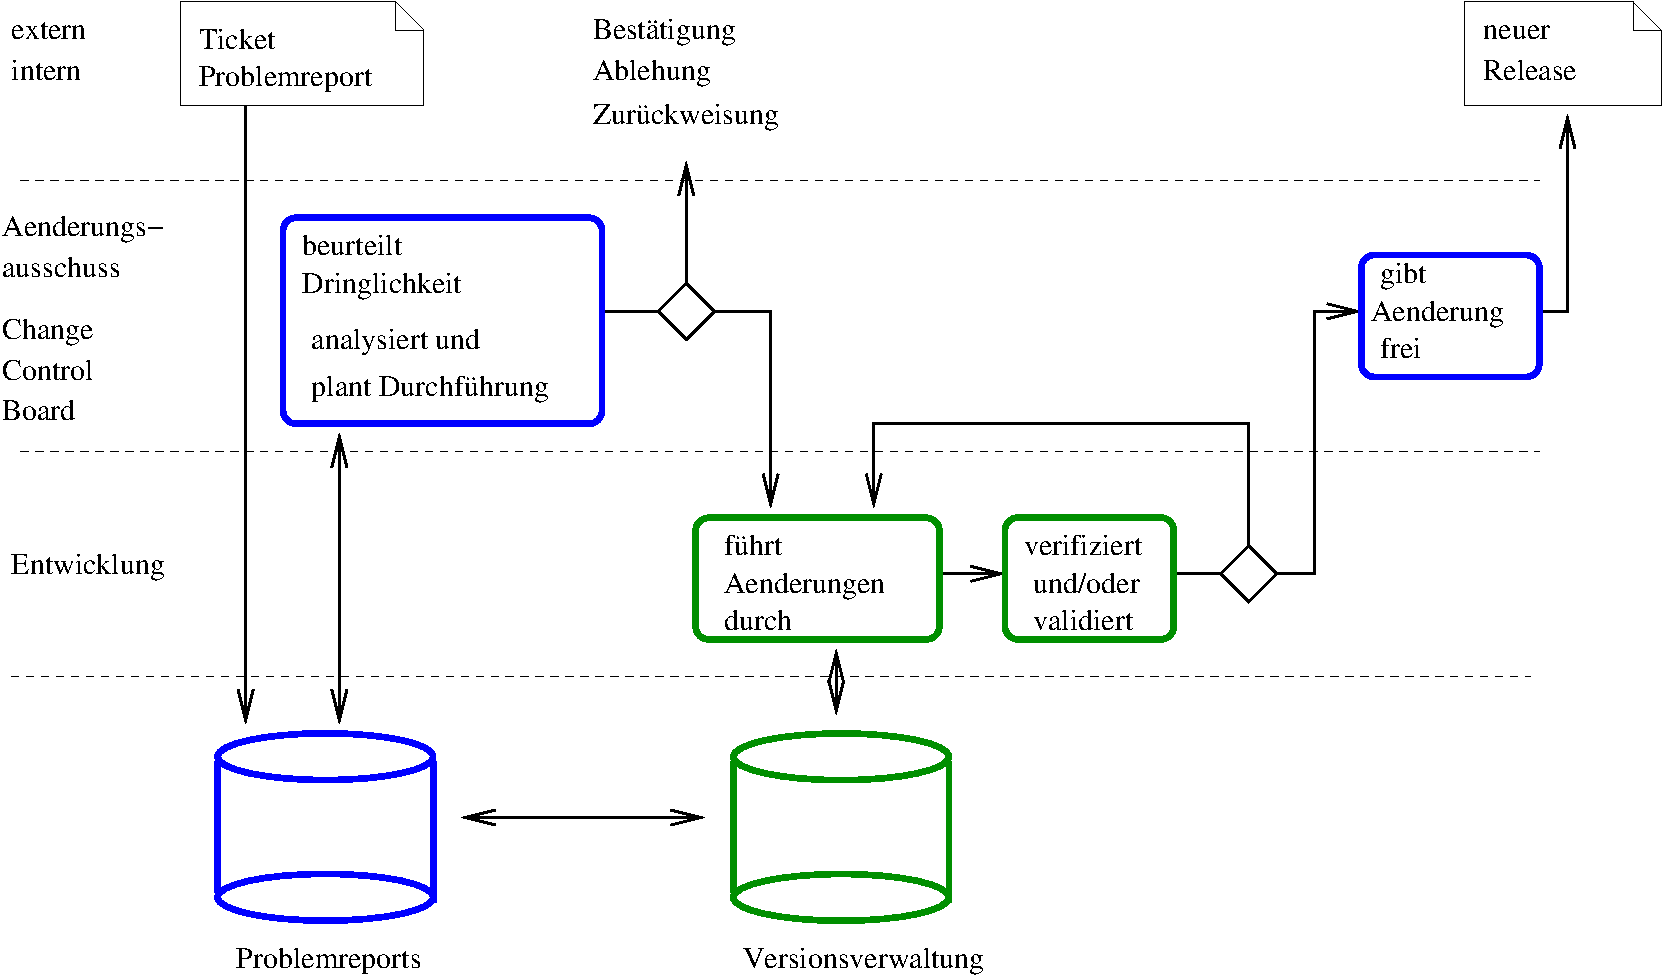
\includegraphics[width=\linewidth]{config-management/xfig/changemgmt}
\caption{Der Änderungsprozess}
\fi
\end{figure}
\begin{minipage}[t]{0.48\linewidth}
\subsection*{Bug and Issue Tracking} %Problembehandlung
\begin{itemize}
\item Erfassung und Verwaltung aller eingehender Fehlermeldungen
  und \"Anderungsanträgen
\item Entscheidung über die Bearbeitung der Meldungen unter Berücksichtigung
 der technischen und zeitlichen Auswirkungen
\item Abschluss der \"Anderung und Information der Betroffenen
\end{itemize}
\end{minipage}
\hfill
\begin{minipage}[t]{0.48\linewidth}
\subsection{Version Control}
\begin{itemize}
\item Eindeutige Kennzeichnung der Software-Elemente
\item Einfrieren von Zwischenergebnissen
\item Sicherstellen dass auf vorangegangene Versionen
  zurückgegriffen werden kann
\end{itemize}
\end{minipage}
\newslide
\section{Software and further Informations}
\begin{itemize}
\item Software Engineering Body of Knowledge (Kap. 7 SCM):
  \href{http://www.swebok.org}{www.swebok.org}
\item Eine nützliche  Linksammlung: \href{http://www.cmcrossroads.com/yp}
                                          {www.cmcrossroads.com/yp/}
\end{itemize}
%---------------------------------------------------------------
\newslide
% CRISP: Complete Repeatable Informative Schedulable Portable
% (Pragmatic Project Automation)
%
